\documentclass[10pt,a4paper]{article}

\usepackage[utf8]{inputenc}
\usepackage[spanish]{babel}
\usepackage[T1]{fontenc}
\usepackage{lmodern}
\usepackage{microtype}

\usepackage{amsmath}
\usepackage{amsfonts}
\usepackage{amssymb}
\usepackage{amsthm}
\usepackage{bm}

\usepackage{graphicx}
%\usepackage[draft]{graphicx}

\usepackage{authblk}

%\usepackage{natbib}
%\bibliographystyle{unsrt}
\usepackage{makeidx}
\usepackage[nottoc,notlot,notlof]{tocbibind}
%\usepackage{color}
%\usepackage{xcolor} % to access the named colour LightGray
%\definecolor{LightGray}{gray}{0.9}
\usepackage{ulem}

\usepackage{array}
\usepackage{booktabs}
\usepackage{multirow}

\usepackage[shortlabels]{enumitem}

%\usepackage [framed, numbered, autolinebreaks]{mcode}
%\usepackage{matlab-prettifier}
\usepackage[cache=false]{minted}
\usemintedstyle{friendly}
\renewcommand\listingscaption{Código}
%\usepackage{listings}
%\renewcommand{\lstlistingname}{Código}

\usepackage{float}
\usepackage{xparse}

\usepackage{siunitx}
\usepackage{physics}
\usepackage{tensor}
%\usepackage{derivative}
\usepackage[thinc]{esdiff}
\usepackage{stackengine}
\usepackage{mathtools}
\usepackage{accents}
\usepackage[version=4]{mhchem}
%\usepackage{pdfpages}


\usepackage[backref=page, colorlinks=true, citecolor=cyan, linkcolor=blue, urlcolor=blue]{hyperref}

%\usepackage{verbatim}


    \makeatletter
\def\@fnsymbol#1{\ensuremath{\ifcase#1\or \dagger\or \ddagger\or
   \mathsection\or \mathparagraph\or \|\or **\or \dagger\dagger
   \or \ddagger\ddagger \else\@ctrerr\fi}}
    \makeatother

\title{TP N°1: Verificación del Rendimiento Térmico de una Caldera}
\author{Ing. Pablo Barral\thanks{\hspace{0.1 em} \texttt{pbarral@fi.uba.ar}.}}
\affil{67.33 Tecnología del Calor}
\affil{Depto. de Ing. Mecánica - FIUBA}
\date{\today \\Revisión 0}

%Realizó: PMB - 23-11-2021
%Mejoras:
%1) Se agregó ejercicio 2.

\newcommand{\g}[1]{\mathbf{\underline{g}}_#1}
\renewcommand{\v}[1]{\mathbf{\underline{#1}}}
\newcommand{\M}[1]{\mathbf{\underline{\underline{#1}}}}

\newtheorem{theorem}{Proposición}[section]
\newtheorem{corollary}{Corolario}[theorem]
\newtheorem{lemma}[theorem]{Lema}

\begin{document}
\maketitle
\tableofcontents
\section{Objetivo}\label{sec:Objetivo}
El objetivo de este trabajo práctico es llevar a cabo el diseño conceptual de una instalación de cogeneración a partir de los requerimientos establecidos por un usuario consumidor de energía térmica y eléctrica. Para ello, se deben generar dos alternativas distintas de cogeneración, y compararlas contra la situación de referencia.
\section{Condiciones}\label{sec:Condiciones}
Los grupos para este trabajo práctico deben ser de dos personas. En el caso de que la cantidad de personas del curso fuera impar, se conformaría un único grupo de tres personas.
\section{Datos}\label{sec:Datos}

Las demandas térmicas y eléctricas de cada uno de los temas se encuentran en la tabla \ref{tab:Datos}.
\begin{table}[ht]
\centering
% To place a caption above a table
%\caption{\textit{Datos de los diferentes temas.}}
\begin{tabular}[t]{llcccccc}
% Table content
\toprule
&&&\multicolumn{5}{c}{\textbf{Tema}}\\
&&&\textbf{1} & \textbf{2} & \textbf{3} &  \textbf{4} & \textbf{5}\\
\midrule
EE&&$\SI{}{MW(e)}$&$1,5$&$20$&$50$&$80$&$20$\\
VAPOR&$p_v$&$\SI{}{bar(g)}$&$12$&$15$&$10$&$12$&$11$\\
&$G_v$&$\SI{}{\frac{t}{h}}$&$4$&$120$&$150$&$150$&$10$\\
&$p_v$&$\SI{}{bar(g)}$&&$7$&&&\\
&$G_v$&$\SI{}{\frac{t}{h}}$&&$70$&&&\\
CALOR&$Q$&$\SI{}{\frac{Mkcal}{h}}$&$4$&&$15$&&$30$\\
&$t_Q$&$\SI{}{\celsius}$&$110$&&$130$&&$300$\\
CONDENSADO&$p_{cond}$&$\SI{}{bar(g)}$&$3$&$4$&$5$&$4$&$3$\\
&$t_{cond}$&$\SI{}{\celsius}$&$95$&$90$&$92$&$70$&$75$\\
&$G_{cond}$&\% de $G_{v_{tot}}$&$40$&$60$&$50$&$70$&$65$\\
\bottomrule
\end{tabular}
% Or to place a caption below a table
\caption{\textit{Datos de los diferentes temas. }}
\label{tab:Datos}
\end{table}

Además, tener en cuenta que:
\begin{enumerate}
    \item El vapor que se consume con fines de uso térmico en el proceso industrial es saturado.
    \item La presión del condensado es de referencia. No tiene un impacto significativo en su entalpía y su verdadero valor depende de las condiciones del bombeo de trasvase, de la altura del tanque de destino y de la presión a la que este se encuentra. En caso de que la presión del tanque que reciba el condensado sea mayor, adecuar este valor.
    \item El vapor que se produce en la situación de referencia\footnote{Situación sin integración.} se produce en una única caldera de baja presión, la cual quema gas natural.
    \item El calor demandado por el proceso es en forma de gases calientes.
    \item El PCI del gas natural considerado es de $\SI{8400}{\frac{kcal}{m^3N}}$.
    \item Si se considera la instalación de una turbina de gas, debe consultarse el catálogo de un fabricante para obtener la potencia de la turbina, su rendimiento térmico, la temperatura de los gases de escape y su caudal.
    \item El agua de alimentación a las calderas (mezcla del retorno de condensado con la reposición al ciclo) tiene que estar desaireada. Para esto, debe estar en un tanque con una temperatura mínima de $\SI{105}{\celsius}$, al cual se le debe inyectar vapor.
    \item No considerar pérdidas de carga en las calderas.
    \item Considerar un $1\%$ de purga si se usa agua desmineralizada en el ciclo, y $5\%$ si se usa agua ablandada.
    \item En caso de que se considere instalar una caldera de recuperación, los valores de ``pinch point'' y de ``approach'' deben ser elegidos.
    \item Las calderas convencionales queman con un exceso de aire del $15\%$.
    \item Las alternativas deben trabajar en condición de ``autogeneración''. Esto es: se debe abastecer toda la demanda térmica, y no es conveniente la exportación de energía eléctrica.
    \item Considerar como precio de la energía eléctrica $\SI{80}{\frac{USD}{MWh}}$ y del gas natural $\SI{160}{\frac{USD}{dam^3N}}$.\footnote{Tener en cuenta que estos valores son variables y dependientes de: las políticas energéticas, la localización geográfica, la coyuntura, los subsidios, si es un precio de compra o de venta, el tipo de mercado eléctrico, el acceso al combustible, etc.}
    \item El rendimiento térmico de la caldera convencional que se adopte debe ser del $90\%$, el abastecimiento de energía eléctrica se hace con un rendimiento del $50\%$, el rendimiento isoentrópico de las turbinas de vapor es del $80\%$, el de las bombas del $70\%$.
    \item Las condiciones del medio de referencia, para el cálculo de la exergía, son de $p_0=\SI{101}{kPa(a)}$ y $\SI{15}{\celsius}$.
    \item Se puede adoptar un calor específico medio para los gases de escape de turbina, de caldera, o bien para el aire. Están disponible en el campus de la materia una herramienta para elegir el valor, con composiciones típicas de los gases de escape de turbina, de caldera y para el aire
    \item Si se abastece de vapor al proceso con la extracción de vapor de una turbina, esta tiene que estar atemperada hasta $\SI{10}{\celsius}$ por encima de la temperatura de saturación a esa presión.
\end{enumerate}






%Hay que plantear tres situaciones: la de referencia y dos soluciones. Siempre en condición de autogeneración y que no es conveniente exportar (se permite únicamente hasta un 5 por ciento de lo que necesito consumir, en caso de necesidad, pero debe ser minimizado
    
    
%    Darles un precio genérico de EE y GN, aclarando que esto es variable a lo largo del país, y en el tiempo, la coyuntura local y global, y las políticas.
    
    
%        \item ver de dar un cp medio para los gases, utilizar de refrencia los cálculos que hice y que subi al campus. Anotar esto, y pedirles que o bien elijan de ahi, o bien elijan las fracciones molares que pongo, o bien elijan un valor promedio, lo que les parezca mejor.
    
    
    
    
    %ver bien los temas. Tratar de que tengan problemas con la turbina de gas. Pensar lo que quería PAE.

%Pensar la instalación cómo respondería ante un incremento futuro de la demanda de vapor y/o de energia eléctrica.

%pensar bien las condiciones de borde. Poner autogeneracion, preguntar en qué cambiaría si pudiera exportar.

%tratar de que no sea automatizado el asunto.
%tratar de que tengan que poner fuego adicional

%tratar de tener problemas que tengan más de una solucion, cosa de que puedan comparar. Distintas presiones de ciclo de vapor.


%Consigna: eleginr los parametros del proceso.
%hacer el pfd, los tres. Marcar claramente cuál es el límite de batería de la usina, y ´cómo

%darles precios
% calcular cuánto se ahorra de emitir el pais

%rendimientos termicos, marginales, y exergeticos

%conclusiones

%tabla de eestados

%considerar que el agua tiene que estar desaireada, y que el vapor tiene que estar atemperado.

%pensar tmabien cinco temas.

%tener uno grande tipo renova
%uno tipo pae para TG
%uno que tenga agua caliente y que sea chico
%uno cantado para TG chica
%verlos por relacion tn de vapor vs EE. Hacer grandes y chicos.
%hacer que tengan consumo en dos presiones.

%ahorro para la industria que instsala la cogeneracion
%ahorro a nivel pais
%algo de emisiones de CO2 a nivel pais, considerando rendimiento termico medio y todo gas natural.


%dar datos de pinch y approach
%hacer el balance térmico en la caldera de recuperacion

%Consumo de Energía Eléctrica: 50 MW(e)
%• Consumo de Energía Térmica: 150 Tn/h de vapor a 12 bar(g) y 15.000.000kcal/h
%a 130°C.
%• Retorno de Condensado: 50% a 95°C
%• Rendimiento de la Caldera de Fuego Directo: 90%
%• Rendimiento del Ciclo Combinado: 50%
%• Rendimiento de la Turbina de Vapor: 80%
%• Poder Calorífico Inferior del Gas Natural: 8400 kcal/Nm3
%• Calor Específico de los Gases de Combustión: 0,24 kcal/K/kg



%Estudios de posibilidades de cogeneración
%1. 5 MW eléctricos, 4 tn/hr de vapor a 12 bar y 4000000 kcal/hr a 120ºC
%Retorno de condensados: 40% a 95ºC
%2. 20 MW e, 120 Tn/hr a 6 bar, 70 Tn/hr a 15 bar.
%Retorno de condensados: 60% a 95ºC
%3. 50 MW e, 150 Tn/hr a 10 bar y 15.000.000 kcal/hr a 130ºC
%Retorno de condensados: 50% a 95ºC
%4. 80 MWe, 150 t/h de vapor a 12 bar. 70% retorno condensados a 70ºC
%5. 20 MW e, 10 Tn/hr a 10 bar y 30.000.000 kcal/hr a 300°C.
%Sin retornos de condensados
%Rendimientos de calderas: 90%
%Rendimiento de ciclo combinado: 50% (en fábrica)
%Rendimiento turbina de vapor, respecto de la evolución isoentrópica: 80%
%Rendimiento de las turbinas de gas natural: buscar en tablas
%Calcular para la situación de referencia el consumo de energía primaria (gas natural),
%rendimiento térmico y rendimiento exergético de la planta y del conjunto planta y ciclo
%combinado.
%Proponer al menos dos soluciones de cogeneración y realizar un análisis de conveniencia
%en base al cálculo en cada caso de rendimientos energéticos, exergéticos y marginales,
%además del ahorro de combustible porcentual y absoluto. 
\newpage
\section{Información para entregar}\label{sec:Info}

Una vez realizado el cálculo y consolidados los resultados, se debe presentar para su aprobación una memoria de cálculo completa que recoja el detalle de los pasos realizados, de la información relevada del plano y de las suposiciones asumidas. Esta memoria de cálculo debe permitir al lector reconstruir por su propia cuenta el procedimiento llevado a cabo.

Esta memoria de cálculo debe contener, como mínimo, la siguiente información:

\begin{enumerate}
    
    \item Densidad \textit{normal} y densidad \textit{estándar} del gas natural quemado en la caldera.
    
    \item $PCI$\footnote{Poder calorífico inferior, o $LHV$ según sus siglas en inglés (lower heating value). Definimos al $PCI$ como el calor liberado por la combustión completa y estequiométrica del combustible con productos y reactivos en condiciones \textit{estándar}. A este calor se le debe restar el calor de vaporización del agua a la temperatura \textit{estándar}.} del gas natural quemado en la caldera. Utilizar el script incluido \href{https://www.unitrove.com/engineering/tools/gas/natural-gas-calorific-value}{aquí}. Expresarlo en $\SI{}{\frac{kcal}{m^3S}}$, $\SI{}{\frac{kcal}{m^3N}}$ y en $\SI{}{\frac{kJ}{kg}}$.
    
    \item Caudal de gas natural quemado en la caldera, adoptando como válido el rendimiento térmico informado por el fabricante.
    
    \item Composición molar (o volumétrica) y másica de los gases de combustión en base húmeda. Masa molar de los gases de combustión. Caudal másico de los gases de combustión. Caudal volumétrico en condiciones \textit{normales} del aire de combustión. Relación gases húmedos-combustible para el exceso informado. Composición molar de los gases de combustión en base seca.
    
    \item Cuadro de temperatura de llama vs. emisividad de la llama. En él deben figurar el resultado para el valor dato, para este aumentado en un $15\%$ y para este disminuido en un $15\%$.
    
    \item Liberación de calor volumétrica y superficial del hogar.\footnote{La temperatura de llama es el único valor que se debe calcular tres veces, para distintas emisividades de llama. El resto de los valores, por ejemplo, las liberaciones de calor, solamente deben calcularse para la emisividad de llama dato.}
    
    \item Cuadro en el que figuren el coeficiente de intercambio térmico por radiación de los gases triatómicos, el coeficiente de transferencia por convección, el coeficiente de transferencia global, el área de transferencia y la diferencia de temperaturas media logarítmica para:
    \begin{itemize}
        \item Tubos pantalla,
        \item Sobrecalentador,
        \item Haz convectivo,
        \item Economizador.
    \end{itemize}
    
    \item Comparación del área necesaria para el sobrecalentamiento con el área dispuesta por el fabricante en el sobrecalentador.
    
    \item Cuadro resumen en el que figure el calor transferido en cada sector de la caldera, y el perfil térmico tanto de los gases húmedos como del agua-vapor (temperaturas a la entrada y salida de cada intercambio).
    
    \item Gráficos $T$ vs. $Q$ y $-1/T$ vs. $Q$. Utilizar como referencia los mostrados en las figuras \ref{im:TQ} y \ref{im:-1/TQ}.
    
    \item Temperatura de chimenea, calor cedido al ambiente en esta y rendimiento térmico obtenido de modo indirecto a partir de este calor. Comparación con el valor informado por el fabricante. Diferencia entre el consumo de combustible informado y el obtenido mediante este cálculo.
    
    \item Rendimiento exergético de la caldera, adoptando como válido el valor informado por el fabricante.
    
    \item Pinch point (y dónde se localiza) y approach point de la caldera.
    
    \item Conclusiones.

\end{enumerate}

\paragraph{Archivos de cálculo:}

En caso de que hayan sido usados scripts o programas, deben incluirse tanto los códigos como los archivos de cálculo. En caso de que sean archivos de \textit{EES}, estos deben entregarse convergiendo.

\paragraph{Unidades:}

En cuanto a unidades, se solicita expresar los caudales molares o volumétricos en $\SI{}{\frac{m^3N}{h}}$ o $\SI{}{\frac{m^3S}{h}}$ según el caso; las presiones del agua-vapor en $\SI{}{bar(g)}$; las temperaturas en $\SI{}{\celsius}$; y los caudales másicos en $\SI{}{\frac{kg}{h}}$. Estas son las unidades habituales en la que estos datos son expresados en la práctica.

\paragraph{Presentación de la información:} Se recomienda utilizar cuadros para presentar la información, ya que son muy cómodos para la lectura. Se desaconseja escribir los reemplazos en las fórmulas. Es suficiente incluir las expresiones, los valores asociados y los resultados obtenidos.


\begin{figure}[ht]
	\centerline{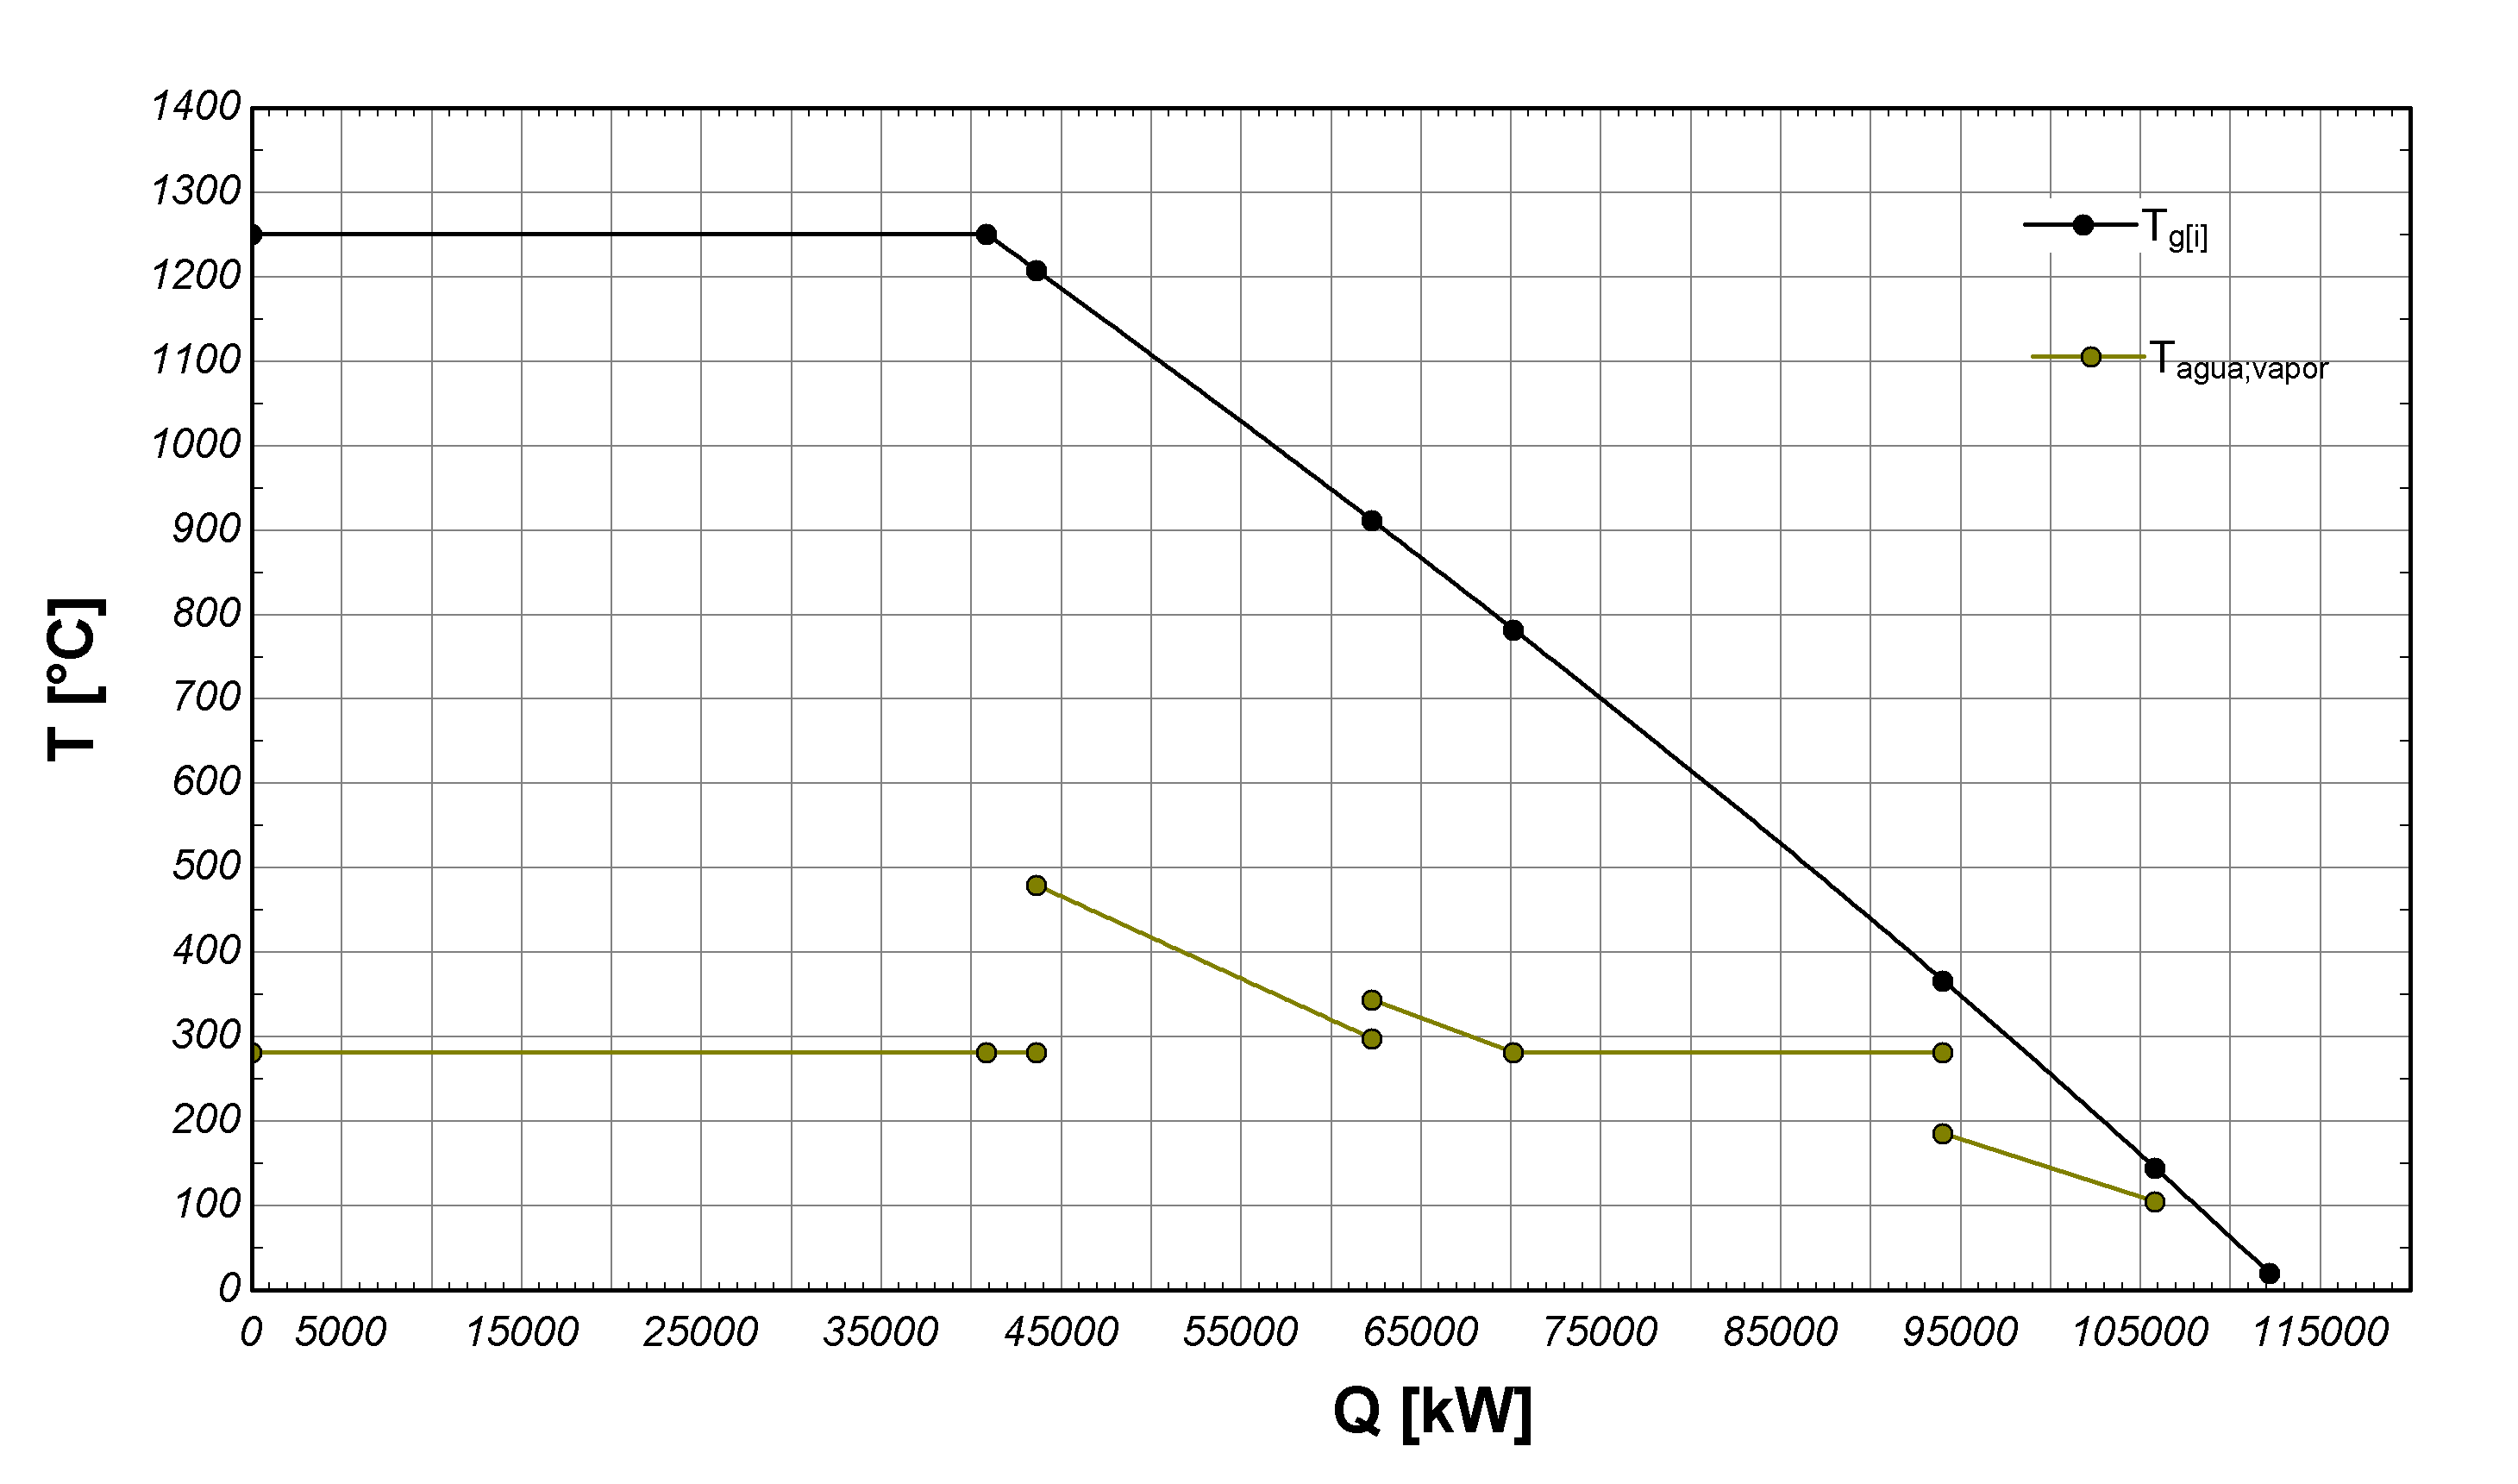
\includegraphics[scale=0.15]{graph_01.png}}
	\caption{\textit{En este caso la curva de la caldera es más compleja que la de este trabajo práctico, ya que el sobrecalentamiento está calculado en etapas, utilizando el área dispuesta por el fabricante, y la caldera tiene una atemperación de vapor intermedia.}}
	\label{im:TQ}
\end{figure}


\begin{figure}[ht]
	\centerline{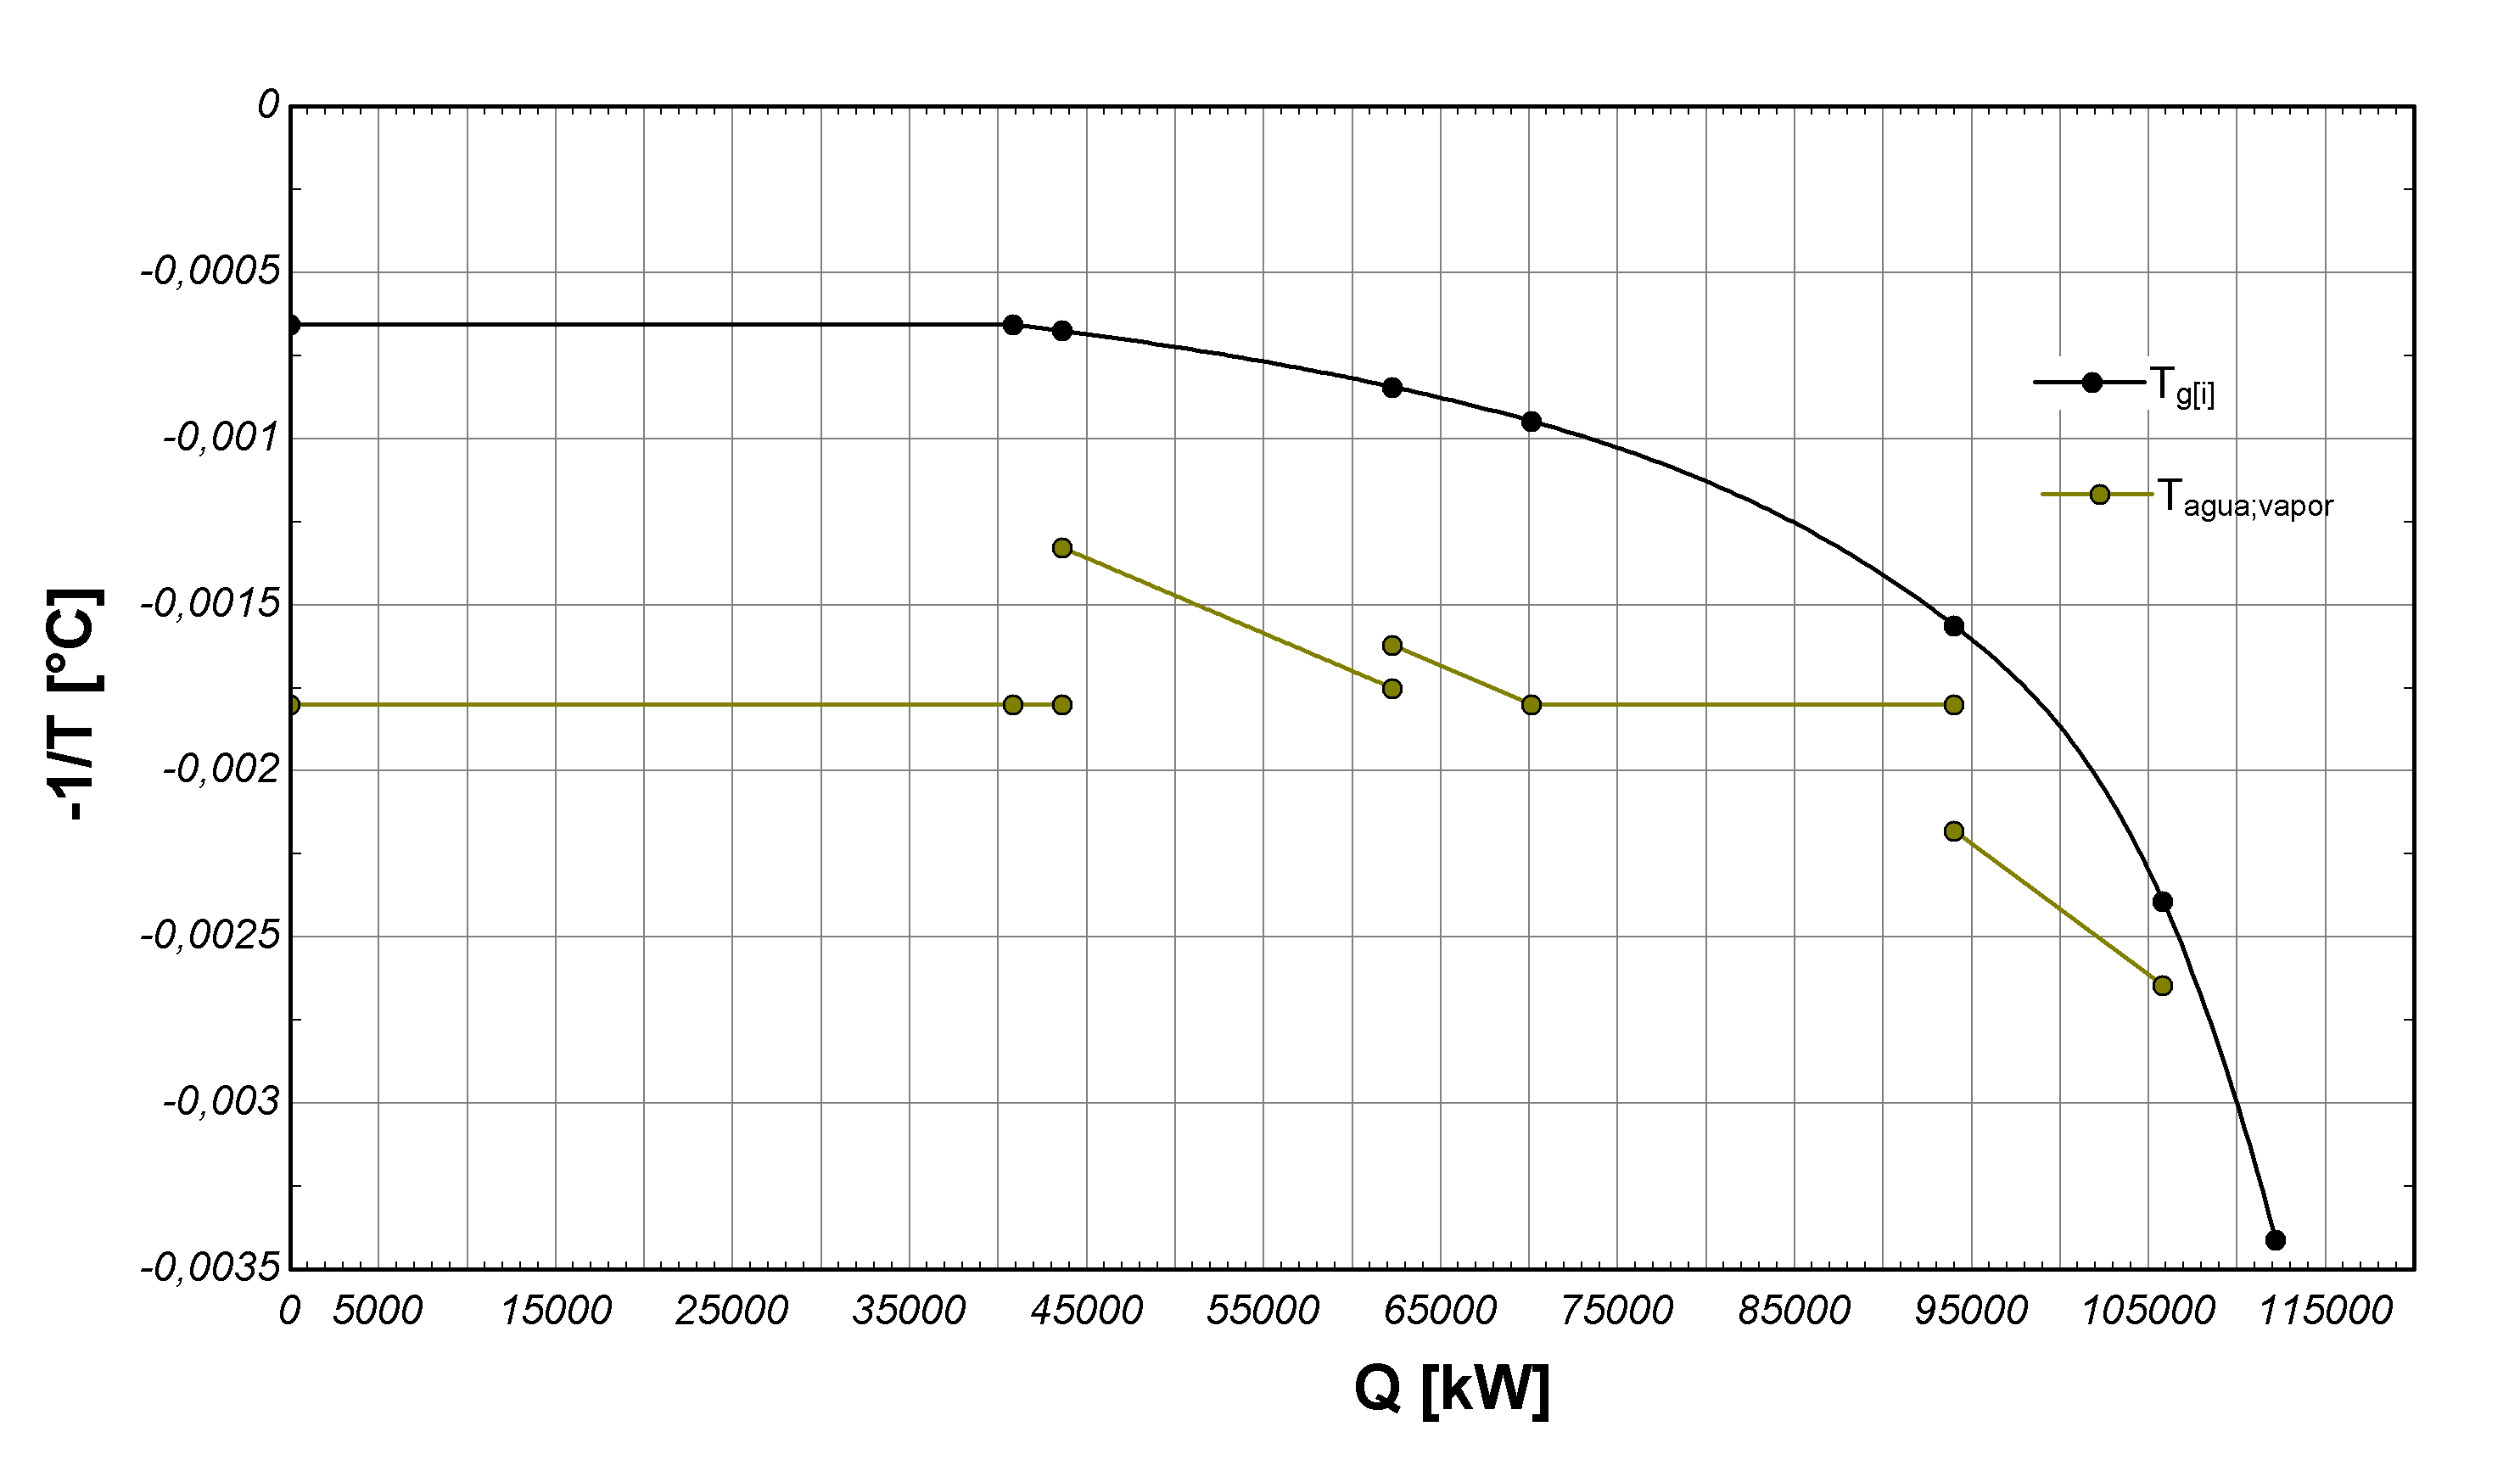
\includegraphics[scale=0.15]{graph_02.png}}
	\caption{\textit{En este caso la curva de la caldera es más compleja que la de este trabajo práctico, ya que el sobrecalentamiento está calculado en etapas, utilizando el área dispuesta por el fabricante, y la caldera tiene una atemperación de vapor intermedia.}}
	\label{im:-1/TQ}
\end{figure}


 





\end{document}

%\includepdf[pages=-,scale=.8,pagecommand={}]{M1}
% embeber archivos EES (fijarle alli los guesses, los limites, las unidades y ponerlo como un pdf
%poner codigos python
%armarles videitos con OBS
% Armarles un buen correo con recursos.
% Poner las cosas en el campus.
% La formula para el schichtdicke del manual de calculo
% La formula del incropera.
% La de pytjon
% Estequiometria
% https://campus.fi.uba.ar/course/view.php?id=525
% VDI G5 G6 M1
%paper de taler
%el de klein
%scripts para estequiometria
% apunte ganapahty

% sacar el PCI usando unitrove.

%https://drive.google.com/drive/u/1/folders/1KMVXKphmClWue-Gjy7hJmKb6AGZ5p6SP

%https://www.unitrove.com/engineering/tools/gas/natural-gas-calorific-value

%llamaremos standard a las condiciones de 15 y 101,325 para diferenciarlo de normal, a 0 y 101,325.